\documentclass[10pt]{article}         %% What type of document you're writing.
\usepackage{graphicx}
\usepackage{hyperref}
\usepackage[dvipsnames]{xcolor}

%%%%% Preamble

%% Packages to use

\usepackage{amsmath,amsfonts,amssymb}   %% AMS mathematics macros

%% Title Information.

\title{INEGI Data Model}
\author{Adolfo Centeno}
%% \date{2 July 2004}           %% By default, LaTeX uses the current date

%%%%% The Document

\begin{document}

\maketitle

\begin{abstract}
This document implements the INEGI Data Model.
\end{abstract}

\section{Data Model Description}


\textcolor{red}{Entidades} de mexico (\textcolor{green}{ identidad, nombreentidad } ) \\
\textcolor{red}{Municipios}  (\textcolor{green}{ idmunicipio, nombremunicipio} ) \\
\textcolor{red}{Empresas}  (\textcolor{green}{ idempresa, nombreempresa, domicilio, tipoactividad [hospital, escuela, oxxo, gobierno, cajero..], latitud, longitud } ) \\

\begin{enumerate}

\item
Las Entidades se \textcolor{yellow}{componen} de Municipios 
\item
Las Municipios  \textcolor{yellow}{tienen} Empresas 

\end{enumerate}


\section{E-R Model}

INEGI...

\begin{figure}[h]
     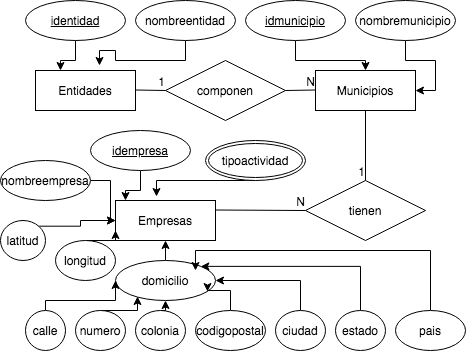
\includegraphics[scale=0.4]{er_inegi}
     \caption{INEGI E-R Model}
\end{figure}
   
\section{Relational Model}
INEGI Relational Model

\begin{figure}[h]
     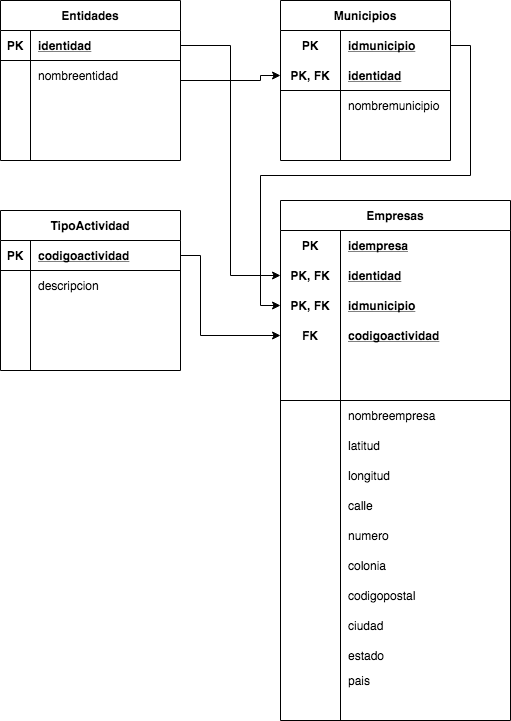
\includegraphics[scale=0.4]{relational_inegi}
     \caption{INEGI Relational Model}
\end{figure}


\section{Database in postgresql}
Database script

\begin{enumerate}

\item
	sudo -u postgres createdb adsoft\_inegi;
\item
	sudo -u postgres psql;
\item
	\textbackslash connect adsoft\_inegi;
\item
	create table entidades(identidad int, nombreentidad varchar(200));
\item
	alter table entidades add constraint pk\_identidad primary key(identidad);
\item
	insert into entidades values (1, 'AGUASCALIENTES'); \\
	insert into entidades values (2, 'BAJA CALIFORNIA'); \\
	insert into entidades values (3, 'BAJA CALIFORNIA SUR');
\item
	create table municipios(idmunicipio int, identidad int, nombremunicipio varchar(200));	
\item
	alter table municipios add constraint pk\_identidad\_idmunicipio primary key(identidad, idmunicipio);
\item
    alter table municipios add constraint fk\_identidad foreign key(identidad) references entidades(identidad);
\item
	insert into municipios values (1, 1, 'EL LLANO'); \\
	insert into municipios values (1, 2, 'TIJUANA'); \\
	insert into municipios values (2, 2, 'MEXICALI');
\item
	create table tipoactividad(codigoactividad int, descripcion varchar(200));
\item
	alter table tipoactividad add constraint pk\_codigoactividad primary key(codigoactividad);
\item
	insert into tipoactividad values(522110, 'BANCA MULTIPLE'); \\
	insert into tipoactividad values(522451, 'MONTEPIOS');
\item
	create table empresas(idempresa int, identidad int, idmunicipio int, codigoactividad int, nombreempresa varchar(200),   latitud float, longitud float, calle varchar(100), numero int, colonia varchar(100), codigopostal int, ciudad	 varchar(100), estado varchar(50), pais varchar(50));
\item
	alter table empresas add constraint pk\_id\_empresa\_identidad\_idmunicipio primary key(idempresa, identidad, idmunicipio);

\item
alter table empresas add constraint fk\_identidad\_idmunicipio foreign key(identidad, idmunicipio) references municipios(identidad, idmunicipio);
\item
alter table empresas add constraint fk\_codigoactividad foreign key(codigoactividad) references tipoactividad(codigoactividad);

\item

insert into empresas values (1, 1, 1, 522110, 'SUCURSAL BANAMEX 1', 21.88234, -102.28259, 'AV 1', 1, 'CENTRO', 98800, 'AGUASCALIENTES', 'AGS','MEXICO');\\
insert into empresas values (2, 1, 1, 522110, 'SUCURSAL BANORTE 1', 21.88287, -102.28242, 'AV 3', 100, 'CENTRO', 98800, 'AGUASCALIENTES', 'AGS','MEXICO');\\
insert into empresas values (3, 1, 1, 522451, 'CAJERO BANCOMER 1', 21.88255, -102.28231, 'AV 9', 20, 'CENTRO', 98800, 'AGUASCALIENTES', 'AGS','MEXICO');

\end{enumerate}


\section{Querys in SQL}

\begin{enumerate}

\item proyeccion:  select field1, field2 .. \\
	select identidad, nombreentidad from entidades; \\
	select nombreentidad from entidades;

\item proyeccion con alias: \\
 	select identidad as id, nombreentidad as estado from entidades; \\
 	select identidad, nombreentidad as estado from entidades;
 	
\item seleccion : \\
	select identidad, nombreentidad as estado from entidades where identidad = 1; \\
	select identidad, nombreentidad as estado from entidades where identidad > 1; \\
	select identidad, nombreentidad as estado from entidades where identidad <= 2; \\
\item selecccion y proyeccion
	select nombreentidad as estado from entidades where identidad <= 2; \\
\item selecccion, proyeccion y alias
	select nombreentidad as estado from entidades where identidad <= 2; \\
\item selecccion, proyeccion, alias y rango \\
	select nombreentidad as estado from entidades where identidad in (2,3);	
\item seleccion con operadores logicos \\
	select * from empresas where identidad = 1 and idempresa = 1; \\
	select idempresa, identidad, idmunicipio, nombreempresa  from empresas where idempresa = 1 or idempresa = 2; \\
	select idempresa, identidad, idmunicipio, nombreempresa, codigoactividad  from empresas where identidad= 1 and codigoactividad in (522110);
\item count: \\
	select count(*) from empresas; \\
	select count(*) as numempresas from empresas; 
	select count(*) as numempresas from empresas where identidad = 1;
\item avg: \\
   select avg(latitud)  from empresas where identidad = 1;
\item sum: \\
   select sum(codigoactividad)  from empresas where identidad = 1;   
\item sum: \\
   select sum(codigoactividad)  from empresas where identidad = 1;   
\item max, min
   select max(codigoactividad)  from empresas where identidad = 1;
   select min(codigoactividad)  from empresas where identidad = 1;   
\item stadistic functions : \\
select count(*), sum(codigoactividad), avg(codigoactividad), max(codigoactividad), min(codigoactividad)  from empresas where identidad = 1;

\item PRODUCTO CARTESIANO 2x2 : \\
 select * from entidades, municipios; \\     
 select * from entidades, municipios where entidades.identidad = municipios.identidad; \\
 select entidades.identidad, nombreentidad, idmunicipio, nombremunicipio from entidades, municipios where entidades.identidad = municipios.identidad;\\
 select entidades.identidad, nombreentidad, idmunicipio, nombremunicipio from entidades, municipios where entidades.identidad = municipios.identidad and entidades.identidad in (2,3);
 
\item PRODUCTO CARTESIANO 3X3 : \\
select * from entidades, municipios, empresas where entidades.identidad = municipios.identidad and (municipios.identidad = empresas.identidad and municipios.idmunicipio = empresas.idmunicipio); \\
select nombreentidad, nombremunicipio, nombreempresa, latitud, longitud from entidades, municipios, empresas where entidades.identidad = municipios.identidad and (municipios.identidad = empresas.identidad and municipios.idmunicipio = empresas.idmunicipio);

\item group by \\
 select identidad, count(*) from empresas group by identidad;\\
 select identidad, count(idmunicipio) from municipios group by identidad; \\
 select codigoactividad, count(idempresa) from empresas group by codigoactividad;

\item order by \\
 select identidad, count(*) as numeroempresas from empresas group by identidad order by count(*) desc; \\
 select identidad, count(idmunicipio) from municipios group by identidad order by identidad asc; \\
 select codigoactividad, count(idempresa) from empresas group by codigoactividad order by codigoactividad asc; 

\item group by, having , order by \\
 select identidad, count(*) as numeroempresas from empresas group by identidad having count(*) = 0 order by numeroempresas asc; \\
 select identidad, count(idmunicipio) from municipios group by identidad having count(idmunicipio) = 1 order by identidad asc; \\
 select codigoactividad, count(idempresa) from empresas group by codigoactividad having count(idempresa) = 2  order by codigoactividad asc; 


\end{enumerate}

\end{document}

